\chapter{Балансировка линии сборочных производств}

\label{ALBP}

% \todo[inline, color=red]{Решение проблем балансировки линии частная задача теории расписаний для сборочных производств?}

\section{Назначение и условия применения алгоритмов плана работы на такт}
\subsection{Назначение плана работы на такт}
На рисунке \ref{ris:optimization} приведена подсистема оптимизации. В предыдущем разделе были рассмотрены методы оптимизации на уровне имитационной модели, в данном разделе будут рассмотрены методы оптимизации на уровне входных данных, то есть предобработка технологической карты.

В связи с тем, что одной из основных целей проделанной работы является оптимизация производственного процесса, в рамках имитационной модели были реализованы оптимизационные задачи. Но как было замечено ранее, подходы к оптимизации не всегда эффективно справлялись со своей задачей, ввиду примитивной, но рабочей реализации (ввиду специфичности данных, с которыми работает имитационная модель). Основная проблема заключалось в сложности исходной задачи, где время работы алгоритмов случайного перебора определяется факториальным временем. Таким образом необходимо знать размер входных данных, и исходя из этого принимать решение о целесообразности применения полного перебора.

Для того, чтобы уменьшить влияние входных данных были разработаны разные вариации алгоритмов составления плана работы на такт. Назначением плана работы на такт является обеспечение максимизации загрузки ресурсов, что приведет к повышению экономической эффективности производства. ПРТ представляет из себя оперативный план на один такт сборочного производства, включающего в себя линии и посты, при полной его загрузке - заготовки находятся на каждом посту каждой линии.

\subsection{Входные данные}
В данном разделе приведена структура данных для алгоритма работы оптимизации плана работы на такт:
\label{assembly_line_balancing:input_data}
\begin{itemize}
	\item[1)] Технологическая карта включает:
		\begin{itemize}
			\item операции и их причинно-следственные связи;
			\item рабочие места на заготовке, макс. кол-во работников на рабочем месте;
			\item задействованные ресурсы для каждой операции:
				\begin{itemize}
					\item[а)] работники соответствующих профессий (min, max, трудоёмкость, диапазон ожидаемого отклонения трудоёмкости\footnote{Позволяет учитывать при планировании ожидаемые отклонения по оптимистическому/пессимистическому/случайному сценарию.});
					\item[б)] рабочее место на заготовке;
					\item[в)] \textit{номер поста для операции};
				\end{itemize}
		\end{itemize}
	\item[2)] Параметры производства включают:
		\begin{itemize}
			\item организация производства:
				\begin{itemize}
					\item[а)] кол-во линий;
					\item[б)] \textit{кол-во постов};
					\item[в)] доступность/недоступность рабочих мест на заготовках на постах\footnote{К примеру, работы на крыше являются высотными и требуют специальных ограждений.};
					\item[г)] \textit{такт производства};
				\end{itemize}
			\item персонал:
				\begin{itemize}
					\item[а)] \textit{макс. кол-во работников в цеху};
					\item[б)] \textit{кол-во работников каждой профессии};
					\item[в)] \textit{привязка работников к посту/линии};
					\item[г)] сменный график по профессиям;
				\end{itemize}
		\end{itemize}
	\item[3)] Настройки расчёта (\textit{опционально}):
		\begin{itemize}
			\item изменение числа работников в процессе работы над операцией:
				\begin{itemize}
					\item[а)] возможность изменение числа исполнителей операции;
					\item[б)] минимальное время участия -- не имеет смысла привлекать работника на очень короткий промежуток времени, так как больше на включение в операцию потратит.
					\item[в)] временные потери на смену рабочего места, включение в выполняющуюся операцию;
				\end{itemize}	
			\item выравнивание сменного графика, производственного такта и операций (по смене, по 1/2, по 1/4, ...);
			\item синхронизация работы линий:
				\begin{itemize}
					\item[а)] задается максимально допустимое время отклонения сборки на одном посту между линиями.
					\item[б)] задается допустимый временной сдвиг между линиями.
				\end{itemize}
		\end{itemize}
	\item[4)] Оценка качества варианта:
		\begin{itemize}
			\item настройка отклонения длительности работы от производственного такта (-0.1, +0.01);
			\item настройки максимальной / минимальной загрузки персонала (0 - особый случай);
		\end{itemize}
\end{itemize}

\subsection{Выходные данные} %%%%%%%%%%%%%%%%%%%%%%%%%%%%%%
Выходными данными является ПРТ, что включает:
\begin{itemize}
	\item[1)] время начала и конца операции (длительность);
	\item[2)] кол-во работников на операцию;
	\item[3)] расписание занятости ресурсов во времени, загрузка;
	\item[4)] временные потери на перемещение персонала (в случае изменения числа работников в процессе работы над операцией).
\end{itemize}


\section{Балансировка сборочной линии}

Производственная сборочная линия была впервые представлена Генри Фордом в начале 1900-х годов. 
Она была разработана с целью повышения эффективности, производительности изготовления конкретного продукта.
Базовая сборочная линия состоит из нескольких рабочих станций, расположенных последовательно, где каждая станция соединена погрузочно-разгрузочным устройством.
Движение материала или заготовки по сборочной линии начинается всегда с первой станции, оно осуществляется с заданной скоростью – она определяется тактом производственной линии.
Станцией может считаться любая точка конвейера, на которой выполняется обработка заготовки - машинами, роботами и или людьми.
Как только заготовка поступает на станцию начинается выполнение соответствующей операции (определяемой технологической картой), после окончания работ она подается на следующую станцию.
Время, необходимое для выполнения операции на каждой станции, называется временем процесса \cite{Sury}.
Цикл производственной линии представляет собой общее время прохождения заготовкой всех станций конвейера с учетом простоев между операциями.
Длительность цикла сборочной линии определяется желаемой производительностью.
Этот уровень производства устанавливается таким образом, чтобы желаемое количество конечного продукта было произведено в течение определенного периода времени \cite{Baybars}.
Для того чтобы сборочная линия поддерживала определенную производительность, такт производственной лини (время самой длительной операции конвейера) не должен превышать среднюю длительность процессов на станциях.
Если время обработки на некоторой станции превышает среднюю длительность операции конвейера, говорят, что на этой станции присутствует простой.
Одним из основных вопросов, касающихся организации сборочной линии, является порядок выполнения задач.
Проблема балансировки сборочной линии (ALBP) возникла вскоре после широкого распространения сборочных линий в промышленности.
Хельгесон и др.
\cite{Helgeson} были первыми, кто предложил рассмотрение ALBP, как проблемы, требующей исследований, тогда как Сальвесон \cite{Salveson} был первым, кто опубликовал предложил математическую формализацию проблемы.
Однако в течение первых сорока лет существования сборочной линии для балансировки линий использовались только методы проб и ошибок.
С тех пор было разработано множество методов для решения различных форм ALBP.
Сальвесон \cite{Salveson} сделал первую математическую попытку, решив задачу в виде линейной программы.
Гутьяр и Немхаузер \cite{Gutjahr} показали, что проблема ALBP относится к классу NP-сложных задач комбинаторной оптимизации. 
Это означает, что оптимальное решение не гарантируется для задач значительных размеров. 
Поэтому эвристические методы стали наиболее популярными методами решения проблемы.



Задачи балансировки линии:

\begin{itemize}
    \item уменьшение количества рабочих станций при заданном цикле;
    \item уменьшение цикла при заданном количестве рабочих станций;
    \item уменьшение общего времени простоя;
    \item уменьшение общего объекта или длины линии.
\end{itemize}

Классификация проблемы ALB основана главным образом на целевых функциях и структуре сборочной линии. Различные версии проблем ALB представлены на рисунке \ref{ris:image1} \cite{Lastra11}.

\begin{figure}[H]
    \center{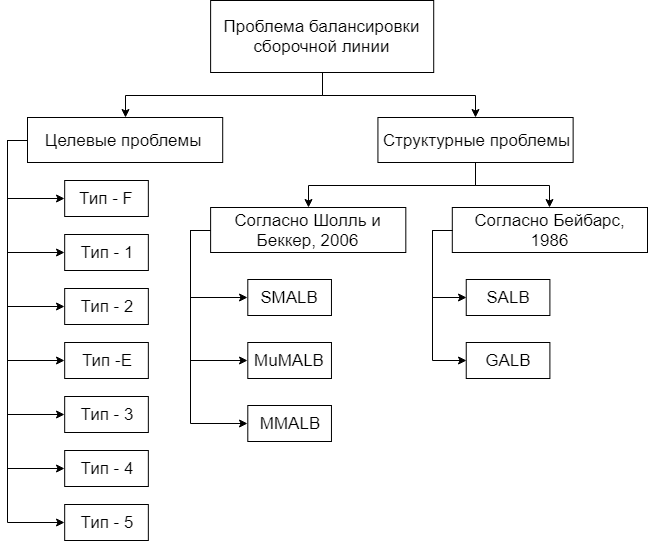
\includegraphics[width=1\linewidth]{fig/ClassALBP.png}}
    \caption{Классификация ALBP}
    \label{ris:image1}
\end{figure}

\subsection{Проблемы базирующиеся на целевых функциях}
В данном подразделе рассматриваются целевые задачи балансировки линии. Далее перечисленные все обозримые проблемы приведенные на классификации \ref{ris:image1} и представленно их краткое описание.
\begin{itemize}
    \item Тип F: Рассматривает возможность создание линии при заданном количестве рабочих станций и цикле.
    \item Тип 1: Рассматривает задачу уменьшения количества рабочих станций, при фиксированном времени цикла.
    \item Тип 2: Рассматривает задачу уменьшения времени цикла, при фиксированном количестве рабочих станций.
    \item Тип E: Данный тип является самой общей версией задачи расчета ПРТ и рассматривает получение максимальной эффективности линии при минимальном цикле и количестве станций.
    \item Тип 3: Рассматривает задачу увеличение плавности рабочей нагрузки.
    \item Тип 4: Рассматривают увеличение синхронности работы, используется в тех случаях, когда нужно производить быстро однотипный продукт.
    \item Тип 5: Рассматривает типы 3 и 4 для нескольких продуктов.
\end{itemize}

В рамках данной работы рассматривается функция повышения эффективности загрузки. Эффективность сборочной линии подразумевает равномерную загрузку всех рабочих станций на сборочной линии. 

\subsection{Проблемы основывающиеся на структуре линии}
В данном разделе рассматриваются структурные задачи балансировки линии. Далее перечислены структурные проблемы приведенные на рисунке \ref{ris:image1} и их описание\cite{Lastra11}.

\begin{itemize}
    \item SMALB: Данная проблема затрагивает структуру, когда на линии производится один тип продукта.
    \item MuMALBP: Затрагивает проблемы производства более одного типа продукта партиями на одной линии.
    \item MMALBP: Затрагивает производство разных типов продуктов на одной линии в любом порядке, без времени переключения (имеется ввиду время необходимое для переоснастки рабочих мест на линии для производства нового типа продукта).
\end{itemize}

\begin{figure}[H]
    \center{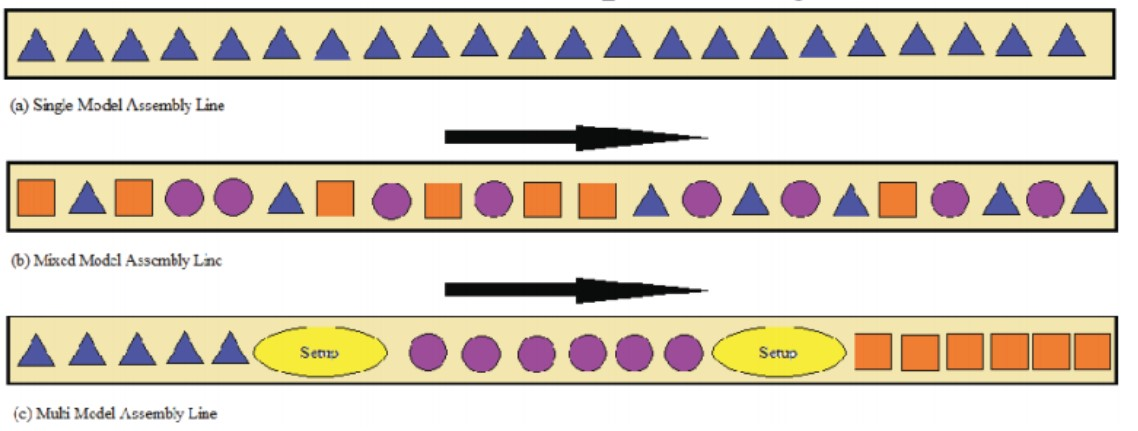
\includegraphics[width=1\linewidth]{fig/Screenshot_2.jpg}}
    \caption{Структура линий из классификации, изображенной на рисунке \ref{ris:image1}}
    \label{ris:shapeOfLines}
\end{figure}

Созданная имитационная модель позволяет игнорировать структурные особенности линии. Основные ограничения, которые невозможно игнорировать включены в технологическую карту. 
% \todo[inline, color=red]{Пока непонятно куда девать время предустановки линии в случае MMALBP}

% Источник: https://ru.scribd.com/doc/7699063/Introduction-of-Line-Balancing



\section{Обзоры методов решения проблем балансировки линии}

На текущий момент известны множество подходов для решения проблемы балансировки линии. Наиболее популярные подходы и методы приведены на рисунке (\ref{ris:Approaches}).

\begin{figure}[H]
    \center{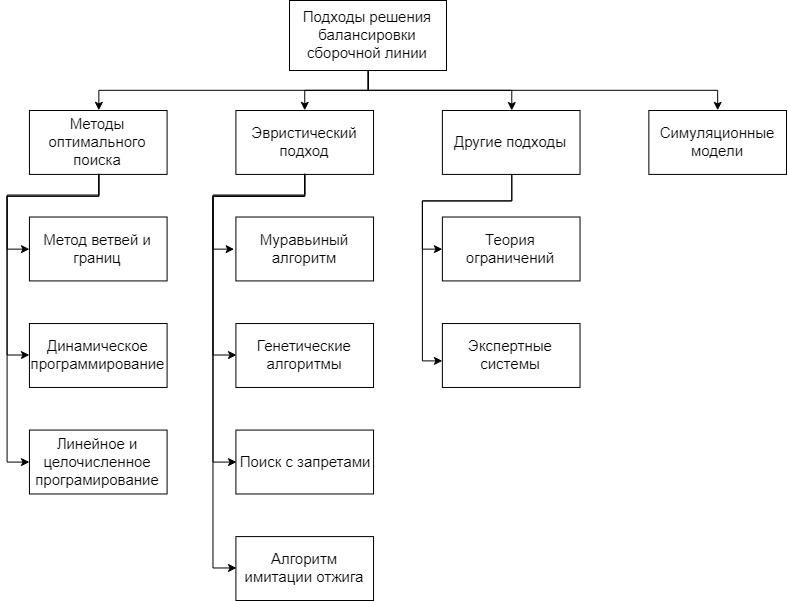
\includegraphics[width=1\linewidth]{fig/Approaches_Rus.jpg}}
    \caption{Различные процедуры решения для ALBP}
    \label{ris:Approaches}
\end{figure}

\subsection{Методы оптимального поиска}
Методы оптимального поиска основаны на математических подходах и позволяют найти из множества объектов оптимальный, который соответствует заданным критериям. Одной из основных проблем данного подхода является вычислительная сложность, что в контексте поиска наилучшей конфигурации конвейера, приводит к существенному ограничению использования методов оптимального поиска. В следующем подразделе будет рассмотрен метод оптимизации случайного перебора, который может существенно снизить вычислительную сложность алгоритма.

\subsubsection*{Метод ветвей и границ}
В общем случае метод ветвей и границ позволяет отсеять подмножество допустимых решений, заведомо не содержащих оптимальных решений. Поиск оптимизируемого подмножества сводиться к поиску станции на которой время выполнения всех операций является максимальным из возможных.

В контексте балансировки линии задача будет сформулирована следующим образом:

\begin{itemize}
    \item[1)] Из всех возможных станций выбор наиболее загруженной с целью полного перебора всех возможных вариантов последовательностей и поиск оптимального решения. В результате может быть два возможных варианта, либо перетасовка операций действительно позволила использовать неиспользуемые ресурсы, либо перетасовка ни к чему не привела. На рисунке \ref{ris:Force} продемонстрированы два варианта разложения технологических карт. 
    
    В первом варианте разложения технологической карты две независимые операции А и В выполняются параллельно при этом задействованы все ресурсы в промежутке от нуля до четырех часов. Далее выполняется операция С, которая требует для выполнения одного работника, при этом трое рабочих остаются без работы на протяжении восьми часов.
    
    Во втором варианте операция С выполняется параллельно с операциями А и В при этом общее выполнения всех операций сократилось до восьми часов и на протяжении 8 часов один незадействованный рабочий.
    
    Данный пример демонстрирует один из возможных способов оптимизации путем перетасовки операций, опирающийся на причинно-следственную связь операций.  Где из всех возможных множеств, выбирается только одно подмножество, которое с большой вероятностью содержит приближенный к оптимальному результат.
    
    \item[2)] В тех случаях, когда оптимизация перетасовки операций не принесла результатов, используется подход основанный на изменении привязок ресурсов к операциям. Так как длительность операции не задается, а рассчитывается на основе входных данных, изменение этих данных позволяет гибко менять длительности операций, и таким образом влиять на загрузку ресурсов. 

\end{itemize}

% \begin{figure}[H]
%     \center{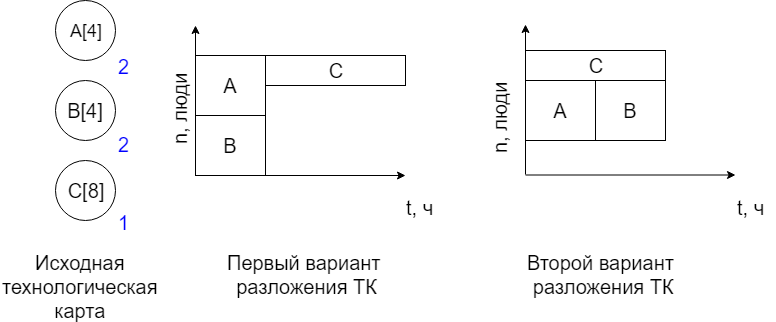
\includegraphics[width=1\linewidth]{fig/DecompositionOfTk.png}}
%     \caption{Различное разложение ТК в зависимости от выбранной последовательности операций}
%     \label{ris:DecompositionOfTk}
% \end{figure}

\subsection{Эврестический подход}

Методы эвристики позволяют нивилировать проблемы комбинаторной сложности задачи, но при этом результат не всегда будет являться оптимальным. Также эффективность работы алгоритмов эвристики во многом зависят от подхода. На рисунке \ref{ris:Approaches} приведены пять различных эвристических алгоритмов, которые использовались для решения проблемы балансировки линии. Одним из наиболее эффективных показал себя генетический алгоритм поиска. Рассмотрим подробно, как работает генетический алгоритм в контексте балансировки линии.

\subsubsection*{Генетический алгоритм}

Генетические алгоритмы хорошо подходят для решения задач планирования производства, потому что в отличие от эвристических методов генетические алгоритмы работают на совокупности решений, а не на одном решении. В производственном планировании эта совокупность решений состоит из множества ответов, которые могут иметь разные, иногда противоречивые цели. Например, в одном решении оптимизировать производственный процесс, который будет завершен за минимальное время. В другом решении оптимизировать для минимального количества дефектов.

По мере того как увеличиваются количество целей, которые пытаемся достичь, также увеличивается количество ограничений на проблему и аналогичным образом увеличиваем сложность. Генетические алгоритмы идеальны для задач такого типа, когда пространство поиска велико, а количество возможных решений мало.

Чтобы применить генетический алгоритм к задаче планирования, необходимо сначала представить каким образом обозначить геном. Одним из способов представления генома планирования является определение последовательности задач и времени начала этих задач относительно друг друга. Каждое задание и соответствующее время его запуска представляют собой ген.

Определенная последовательность задач и времени начала (гены) представляет один ген в нашей популяции. Чтобы убедиться, что геном является возможным решением, надо чтобы он соответствовал ограничениям приоритета. Далее генерируется начальная популяция, используя случайные времена начала в пределах ограничений предшествования. С помощью генетических алгоритмов берется начальная популяция и скрещивается, комбинируя гены с небольшим количеством случайности (мутации). Потомки этой комбинации выбираются на основе функции приспособленности \footnote{Функция приспособленности — вещественная или целочисленная функция одной или нескольких переменных, подлежащая оптимизации в результате работы генетического алгоритма, направляет эволюцию в сторону оптимального решения. Является одним из частных случаев целевой функции}, которая включает одно или много наших ограничений, таких как минимизация времени и минимизация дефектов. Данный процесс продолжаться либо в течение заранее выделенного времени, либо до тех пор, пока не найдется решение, которое соответствует минимальным критериям. В целом каждое последующее поколение будет иметь более высокую среднюю пригодность, то есть займет меньше времени с более высоким качеством, чем предыдущие поколения. Также может потребоваться добавить дополнительные значения пригодности, такие как минимизация затрат; однако каждое добавляемое ограничение значительно увеличивает пространство поиска и уменьшает количество подходящих решений.

\subsection{Результаты экспериментов оптимизации плана работы на такт}
Оптимизация плана работы на такт, в отличии от оптимизации на уровне имитационной модели, работает над обработкой исходной технологической картой. Данное отношения подходов можно увидеть на рисунке \ref{ris:optimization}, демонстрирующей подсистему оптимизации. 

Результаты работы алгоритмов ПРТ, как и в разделе \ref{experiment}, были протестированы на реальных данных. 
Полученные результаты ничего не показали. Это связано с тем, что в привязках к операциям полностью отсутствовала вариативность, число рабочих на операции было строго фиксировано. Таким образом протестировать эффективность алгоритмов ПРТ на реальных данных оказалось невозможным, поэтому для тестирования была создана искусственная ТК.

Основной целью алгоритмов ПРТ была оптимизация конвейеризированных производств. Для этого были разработаны и протестированы два подхода. 
Первый подход заключался в оптимальном поиске случайным перебором. Методом оптимизации случайного перебора был выбран метод ветвей и границ, который значительно уменьшал размер входных данных.
На тестовой ТК алгоритм оптимального поиска показал себя эффективным ввиду небольшого размера исходной задачи.
При этом генетический алгоритм показал подобный результат, при этом была выдвинуто предположение о том, что при большом размере входных данных будет большая разница в эффективности данных подходов в пользу генетических алгоритмов.

